\section{Approaches}
\subsection{Casper Network Topology}
Constructive neural networks are constructive because they will change the architecture of themselves when loss is no longer improved. Here firstly Casper networks start as a simple fully connected network with only input and output layer in Fig.1.1. It’s obvious that such a vanilla fully connected one-layer neuron network is usually not expressive enough to extract the features in training data. Once the loss is non-decreasing, the Casper will add a new neuron into the network. Compared to Cascor, Casper will not freeze previous additional neurons and set difference learning rate to each weight. In Fig.1.2, we can see the difference of each learning rate: L1, L2 and L3. Generally, the value of L1, L2 and L3 are 0.2, 0.005 and 0.001 referring to the technique paper. Learning rate of weights connected to the latest neuron will be set to L1 since the latest neuron is expected to be the feature extractor, and a larger learning rate can speed up the feature learning process. Similarly, the new extracted feature output should reduce the loss without too much interference from the previous weights ~\cite{CascadeCorrelation1990}. Hence it should be set to L2 which is slightly larger than the L3. Since no neurons are frozen, the previous neurons can still be modified if it’s necessary and beneficial. Then the model can both obtain the benefit of the weight freezing and the correlation techniques of Cascor, while avoiding early poor hidden neurons due to weight freezing and the saturation problems due to correlation measure. ~\cite{vae2020}\\

\begin{figure}[hbt!]
\centering
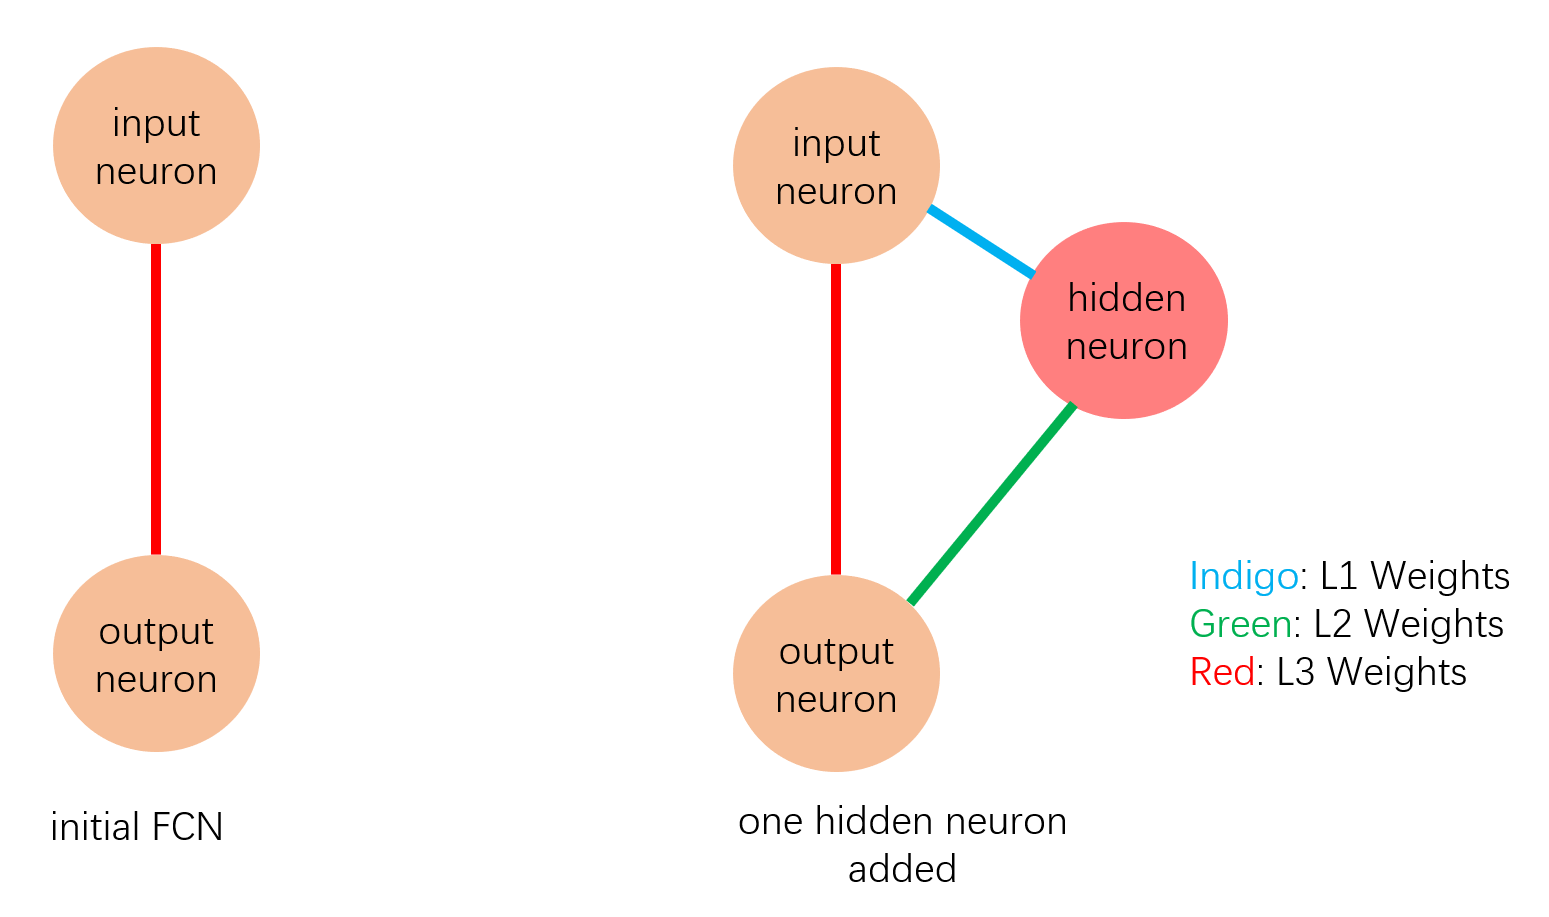
\includegraphics[width=\textwidth]{images/reimg1.png}
\caption{The process to add a random hidden neuron into the network}
\label{figure1}  
\end{figure}

As is shown above in Fig2., it is almost the same when the model add another neuron into the network. Input neuron to 2nd hidden neuron and 1st hidden neuron to the 2nd hidden neuron use the largest weight to significantly change their value to learn features. L2 learning rate is used for the weight between 2nd hidden neuron to the output neuron, which is the output of the latest neuron and needs to give out a more flexible output than previous outputs. In general, the weights connect between input, the previous hidden neurons and the latest hidden neuron share the largest L1 learning rate, and L2 learning rate is used for the weight connects between the latest hidden neurons to the output, which is larger than L3. Therefore, the rest weights perform L3 weight which is the smallest and difficult to change its state.\\
\begin{figure}[H]
\centering
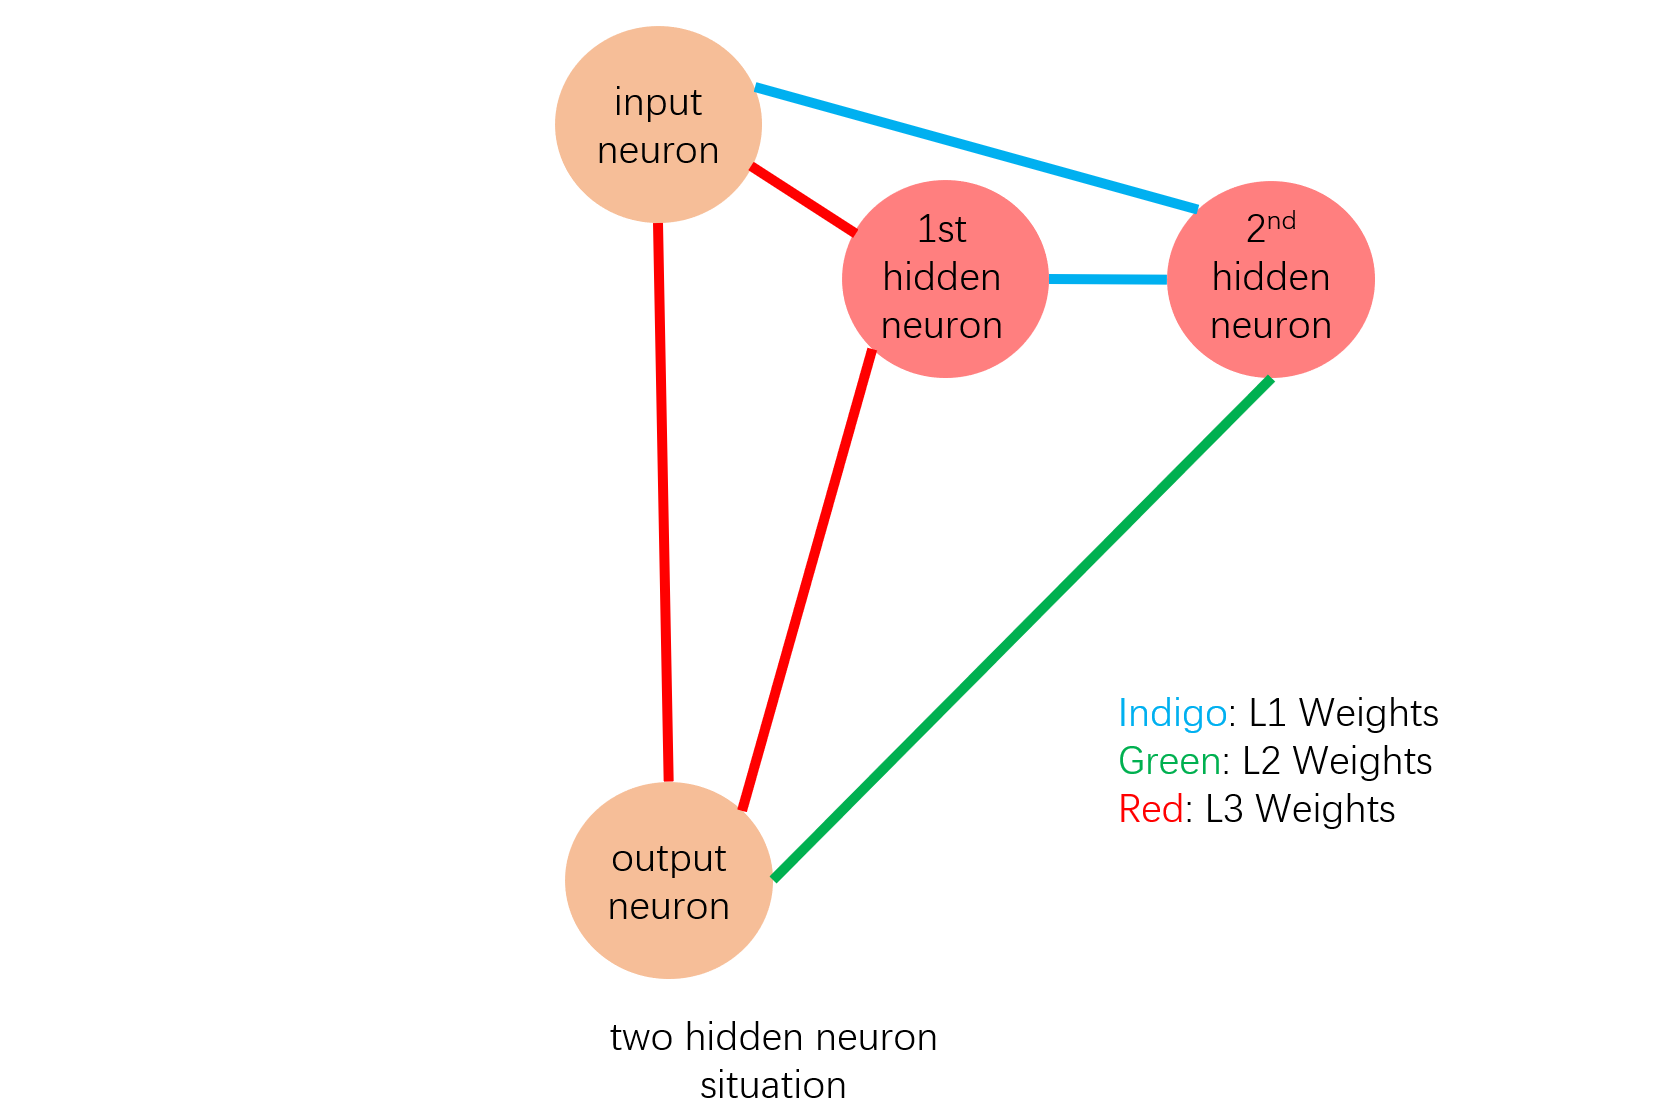
\includegraphics[width=\textwidth]{images/reimg2.png}
\caption{The process to add another hidden neuron}
\label{figure2}  
\end{figure}

\subsection{Conditional Variational AutoEncoder}
AutoEncoder is usually used to find efficient data encodings in an unsupervised manner. Variational AutoEncoder, or in short VAE, are a subclass of AutoEncoder~\cite{vae2020}. VAE provides a probabilistic manner for describing an observation in latent space. Thus, rather than encode the data to a single vector to compress information, we try to make use of the probability distribution to generate data. Here normal distribution is assumed for the following SARS-CoV Dataset. This is quite beneficial if the raw data has large variance and large dimension. A standard VAE should have the architecture in Fig.3. The data is compressed to its latent vector representation by variational encoder. The major difference between variational encoder and standard encoder is reparametrizing data to find the best mean and variance of latent distributions instead of finding latent representations blindly. Hence the latent vector is sampled from the latent calculated distributions in encoder. Thus, the decoder can sample the latent vector from the latent distributions to reconstruct the original data.\\
\begin{figure}[hbt!]
\centering
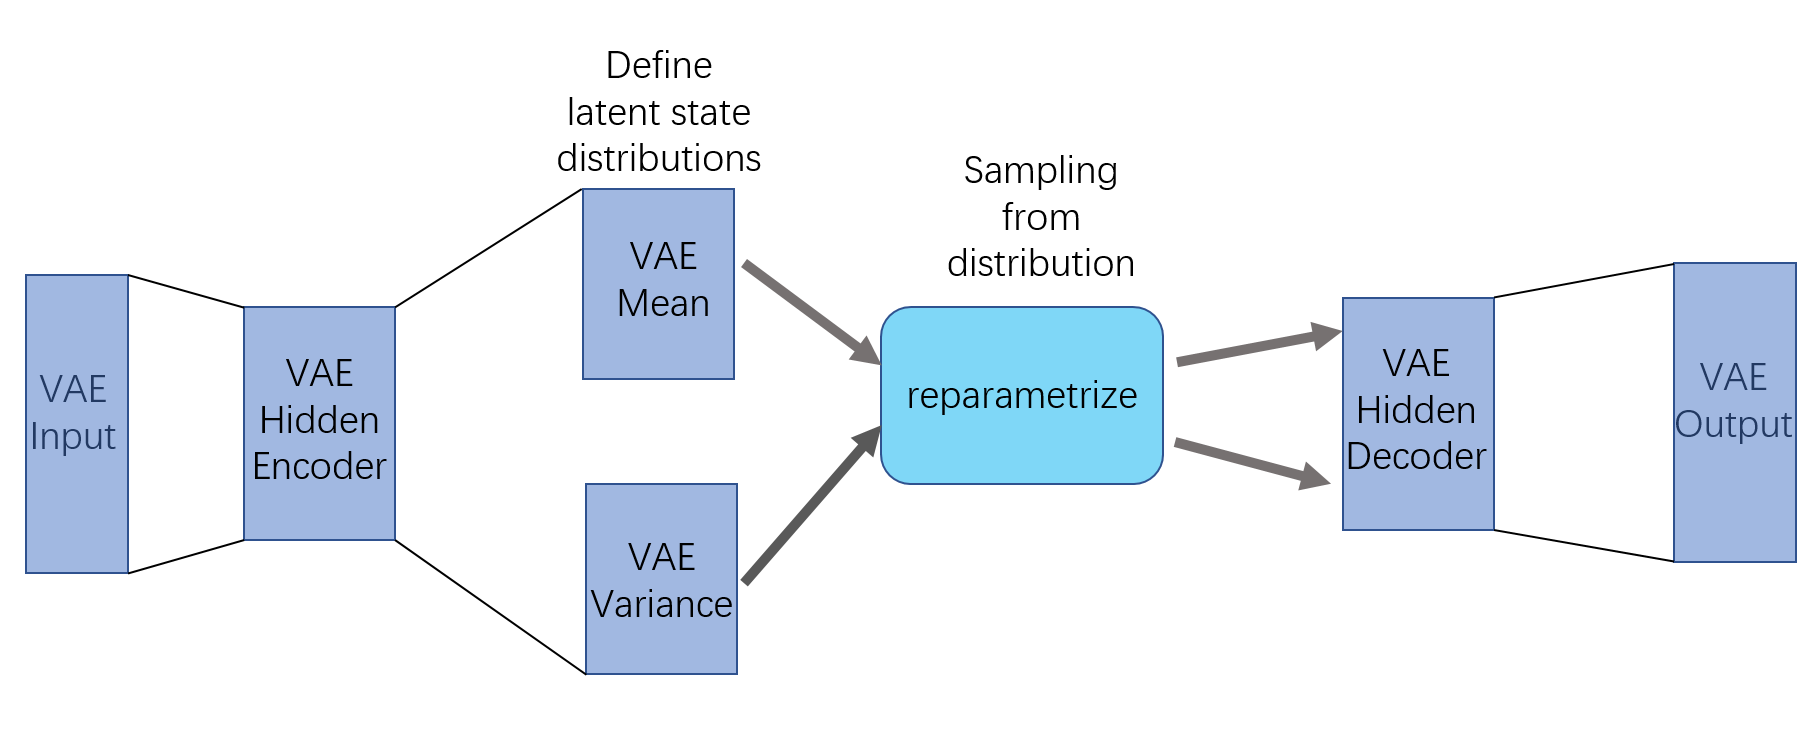
\includegraphics[width=\textwidth]{images/reimg3.png}  
\caption{Vanilla VAE architecture}
\label{figure3}  
\end{figure}

For Conditional VAE ~\cite{cvae}, we can condition the encoder and decoder of VAE to force the model to find different latent space by classes. In other words, we condition all latent distributions with a conditional label $\mathbf{c}$. The conditioning label c is the difference between conditional VAE and vanilla VAE and the latent distribution space becomes: $P(z|c)$ instead of $P(z)$, as the conditional objective is shown below.
$$  
\log P(X \mid c)-D_{K L}[Q(z \mid X, c) \| P(z \mid X, c)]=E[\log P(X \mid z, c)]-D_{K L}[Q(z \mid X, c) \| P(z \mid c)]
$$
\begin{figure}[hbt!]
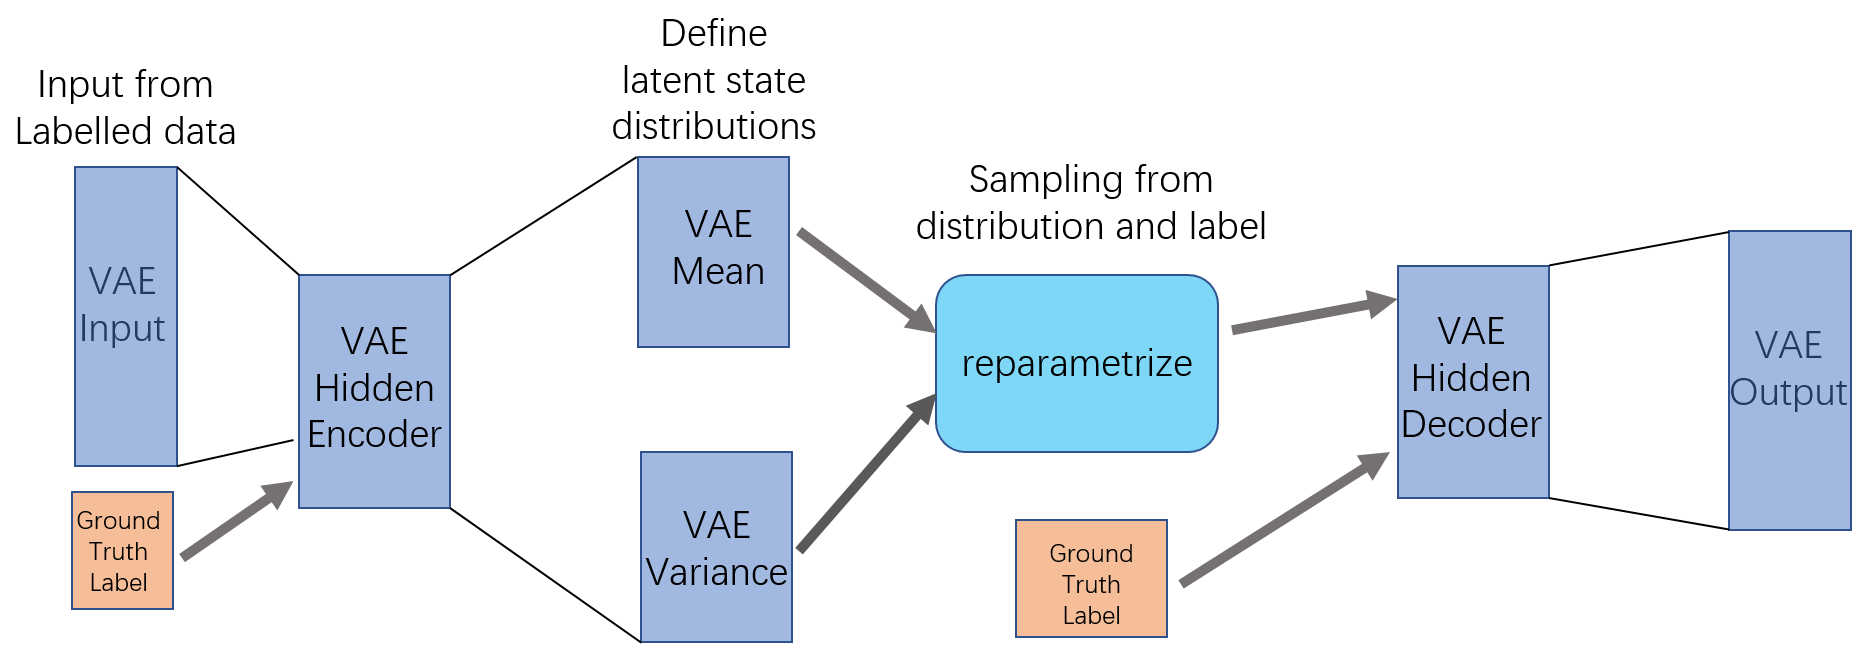
\includegraphics[width=\textwidth]{images/reimg4.png}  
\caption{Conditional VAE architecture}
\label{figure4}  
\end{figure}

Therefore, generative data by conditioning corresponding label can be retrieved from conditional VAE.
\section{Training Pipeline}
The training pipeline we introduce here is as follows. The first module is the CVAE module. Firstly the training data with label is used to train the Conditional VAE module. Since it's Conditional VAE that can generate similar data given labels, we will let CVAE module generates augmentation data given labels we need. Here we choose to generate data four times size larger than the training data. The labels are uniformly distributed while generating. After CVAE comes Casper module, and the Casper makes use of both the original training data and the generated data to train. \\ 
\begin{figure}[H]
\centering
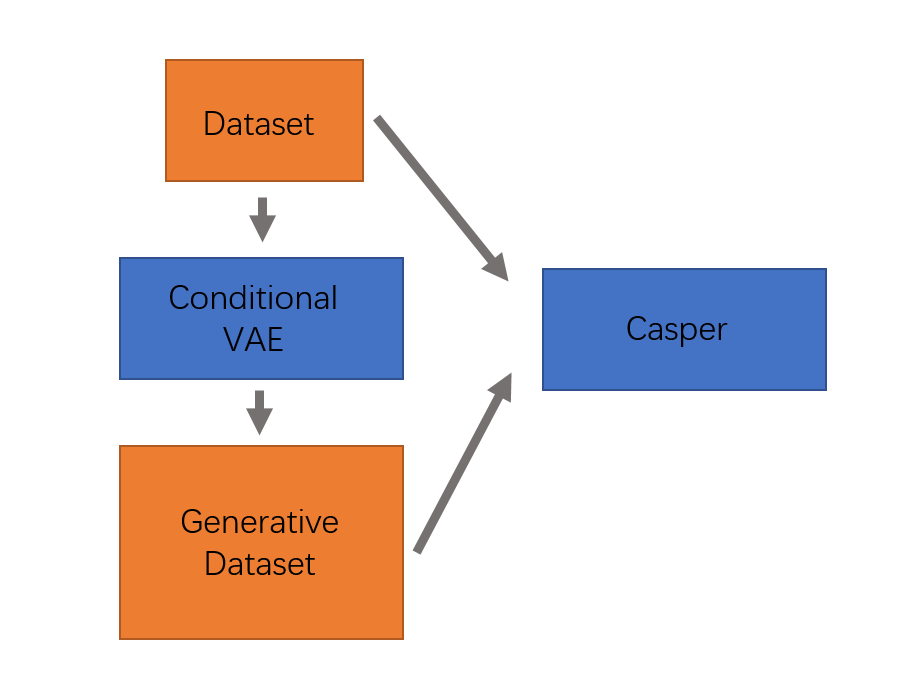
\includegraphics[width=\textwidth]{images/reimg5.png}  
\caption{Training pipeline}
\label{figure5}  
\end{figure}
